\chapter{Results -- Implementation}

\label{ch:implementationresults}

This chapter provides the implementation of the \term{features} of the implemented agents. It will start with the \term{possible vectors} that are sent to any agent and can be used. Afterwards, the agents that where implemented in the scope of this thesis are explained, including all their features and why they were selected this way. These features include the used \codeobj{model}s, the exploration-functions, their specific observation-functions (using the \term{possible features}), their methods of incorporating pretraining as well as their reward-functions. 

It is worth to note, that some of these functions (as for example the \codefunc{calculateReward(gameState)} function) are implemented not in the individual agent, but in \codeobj{AbstractRLAgent}, as they would otherwise have to be redundantly implemented multiple times.

%############################################################################################
\section{Possible vectors}
%############################################################################################

\label{ch:thevectors}

%-progressvec (progress, laptime, lapcount, validvec)
%-speedsteer (motortorques, steerangle, velocity, fRightDirection, velocity of perpendiculars, angle, speedinstreetdir, speedintraversedir, cuvinessbeforecar)
%-carstatusvec (longitutinal and latidutialn slip for each tire)
%-centerdist, als vector
%-waldistvec (direction the car faces, steers, moves..... and directiont the street goes (each longsighted and shortsighted from car and streetmiddle)
%-lookahead-vector
%-delta und feedback
%-actual action (possibly overwritten)
%-both vision-vectors

\term{Possible Vectors} refers to all information the game streams over its socket to the agent. While most of this information will be used to make up an agent's state, the vectors also provide information about if the game must be reset as well as information to calculate the reward from. This information is collected in Unity in the function \codefunc{GetAllInfos()}, and converted into a namedtuple-wrapper called \codeobj{Otherinputs}, specified in \filename{read\_supervised.py}. In this section, I provide an overview of those vectors and their meaning in the game. I refer to the individual possible vectors by the name used in \codeobj{Otherinputs}.

\paragraph{ProgressVec} This vector contains information about the current progress of the car on the track, which consists of the actual progress in percent, the time the car needed for the current lap so far, the number of the current lap, as well as the flag if the round is still \keyword{valid}.

\paragraph{SpeedSteer} In this vector, information about the car's velocity and its steer angle is encoded. It consists of the following values:

\renewcommand{\arraystretch}{1.3}
\begin{flushleft}
	\begin{tabular}{>{\em}p{2.9cm} p{\textwidth-3.8cm}} 
		RLTorque & The motor torque applied to the left back tire\\
		RRTorque & The motor torque applied to the right back tire\\
		FLSteer & The steering angle of the front left tire\\
		FRSteer & The steering angle of the front right tire\\
		velocity & The velocity of the car as scalar independent of directions\\
		rightDirection & A boolean value if the car moves into the intended direction\\
		velocityOfPerpendicular & \hspace*{0.8cm} The velocity of the orthogonal projection of the car onto the center of the street\\ %TODO see sectionbalabla, wo ich DOCH die definition von perpendicular einführen werde
		carAngle & The car's angle (in degrees) in relation to the street's direction\\
		speedInStreetDir & The car's velocity into the street's direction (calculated using the dot-product between the car's velocity-vectors and the direction-vector of the street at the car's current position)\\
		speedInTraverDir &  The car's velocity into the orthogonal of the street's direction\\
		CurvinessBeforeCar & A measure of the curvature of the street immediately ahead of the car ($CurvinessBeforeCar \in [0,1]$, where a value of zero corresponds to a straight street)\\	
	\end{tabular}
\end{flushleft}

\paragraph{StatusVector} This vector contains eight values, corresponding to the forward slip and sideways slip of each of the car's tires, using a function provided by Unity's \codeobj{WheelCollider}-object. The more the car slips, the smaller the impact of movement commands. The current slip-values are presented in the GUI of the game (and can be seen behind annotation \textbf{R} in figure~\ref{fig:aidriveshot}).

\paragraph{CenterDist and CenterDistVec} The \emph{CenterDist} corresponds to the car's orthogonal distance to the street's center in the form of the \keyword{perpendicular} (also visually represented in the car's GUI, behind annotation \textbf{N} in figure~\ref{fig:aidriveshot}).
The \emph{CenterDistVec} contains the same information presented in another way: It is a vector of length 15, where the middle element corresponds to the car's longitutional position. The other elemnts correspond to points with regular distances to the car's left and right. The value of each respective element is calculated using the reversed distance between this position and the longitudional center of the street. The content of this vector is visually represented behind annotation \textbf{M} in figure~\ref{fig:aidriveshot}.

\paragraph{WallDistVec} This vector contains seven values, corresponding to the car's distance to the wall along a certain ray. It does not contain the closest distance to the wall -- because this value is already represented by the CenterDist. As the wall has always a fixed distance from the street's center (with an absolute value of five), the distance to the closest wall can be calculated as $5 - abs(CenterDist)$. 
For the calculation of the \emph{WallDistVec}, several rays are casted from the car's (or the perpendicular's) position into a particular direction. Returned is then the distance from their respective origin and their first intersection with a wall. The vector contains seven values, using rays with different origins and different directions. In the following table, I provide an explanation of each of those values, while figure~\ref{fig:walldistvec} in appendix~\ref{AppendixB} visually represents these rays. The respective color is mentioned in the table.
\renewcommand{\arraystretch}{1.3}
\begin{flushleft}
	\begin{tabular}{p{0.5cm} p{2cm} p{2.4cm} p{\textwidth-6.45cm}} 
		\# & color in \ref{fig:walldistvec} & origin & direction \\
		\hline
		1 & \textcolor{black}{black} & car's center & direction the car faces \\
		2 & \textcolor{magenta}{magenta} & car's center & direction the car steers\\	
		3 & \textcolor{red}{red} & car's center & direction the car moves\\	
		4 & \textcolor{black}{white} & car's center & short-sighted direction of the street (calculated as the vector between the closest \codeobj{anchorVector} behind the car and the closest one before the car) \\		
		5 & \textcolor{yellow}{yellow} & perpendicular & short-sighted direction of the street (calculated as the vector between the closest \codeobj{anchorVector} behind the car and the closest one before the car) \\
		6 & \textcolor{blue}{blue} & car's center & long-sighted direction of the street (calculated as the vector between the closest \codeobj{anchorVector}  to the car and the one 5 in advance) \\
		7 & \textcolor{gray}{gray} & perpendicular & long-sighted direction of the street (calculated as the vector between the closest \codeobj{anchorVector}  to the car and the one 5 in advance) \\
	\end{tabular}
\end{flushleft}

\paragraph{LookAheadVec} This vector corresponds to the course of the street ahead of the car. It is a 30-dimensional vector, corresponding to regularly spaced \codeobj{anchorVector}s, starting at the position of the car, following the direction of the street. The value at each position $i$ of this vector corresponds to the angle between the direction of the street at position $i$ and the direction at position $i+1$. In other words, if the street makes a shart turn 4 units ahead of the car, then element $3$ will contain a high value. The angle is measured in degrees. A graphical representation of this vector can be seen behind annotation \textbf{N} in figure~\ref{fig:aidriveshot}.

\paragraph{FBDelta} This vector consists of two values, namely \emph{Feedback} and \emph{Delta}. The Feedback-value is the temporal difference of how long the car needed for a specific section of the course (constrained via the a \codeobj{anchorVector} close to the car) in the current process in comparison to the time needed in the fastest lap so far. The Delta-value is the absolute difference in time needed for the entire lap so far.

As both of these values are only useful in relation to the time needed for the fastest lap, it must be ensured that this does not change during training. For that, The file \filename{AiInterface.cs} contains in its class \codeobj{Consts} a flag \codeobj{lock\_fastestlap\_in\_AIMode}. Note however, that even if this flag is set, the values of \emph{FBDelta} could at most be used to calculate the agent's reward and not as part of its state.

\paragraph{Action} This is a three-dimensional vector corresponding to the actual action the environment recorded. While the agent knows what action it provided, it could be manually overwritten (after the press of \keystroke{H}) -- which is why the agent stores this vector in its replay memory instead of the action it would have performed otherwise.


\paragraph{minimaps} While the minimaps are not contained in the namedtuple \codeobj{Otherinputs}, their value is transmitted from the game just like the other vectors. In the current implementation, both cameras have a resolution of $30\times45$ pixels, where one camera is $15$ units away of the car, and the other one $75$ units, which means that the former provides a smaller but more detailed view of the car. The closer camera is mostly referred to as $vvec2$, whereas the other one is denoted $visionvec$ or $vvec$.\\

As a working game was already provided by \leon of this thesis, so were some of these vectors, namely the calculation of FBDelta, LookAheadVec, CenterDist and CenterDistVec.

It is worth noting that most \term{possible vectors} are normalized after loading, according to (in part estimated) minimal- and maximal values, such that all their values in [0,1]. The corresponding \codeobj{MINVALS} and \codeobj{MAXVALS} are defined in \filename{read\_supervised.py}

%############################################################################################
\section{Implemented models}
%############################################################################################

Within the context of this thesis, two different models were developed that can be used for agents to learn and play the given game: a \keyword{Double Dueling Deep-Q-Learning} model, specified in the class \codeobj{DDDQN\_model} in \filename{models/dddqn.py}\footnote{\url{https://github.com/cstenkamp/BA-rAIce-ANN/blob/master/models/dddqn.py}} as well as a \keyword{Deep Deterministic Policy Gradient} model, specified in \codeobj{DDPG\_model} in \filename{models/ddpg.py}\footnote{\url{https://github.com/cstenkamp/BA-rAIce-ANN/blob/master/models/ddpg.py}} The theory of the model was explained in chapters~\ref{ch:DQN}ff and \ref{ch:ddpg}, respectively. 

Both models can take two-dimensional as well as one-dimensional input and return outputs corresponding to the action that needs to be taken, which are three real numbers. One has to be aware though that while a DDPG-model can naturally return such, a DQN-model only works for discrete actions. Because it was developed with DQN-models in mind, the \codeobj{AbstractAgent} contains functions to \codefunc{discretize} the action-value returned by the game to a one-hot vector to be used by the model, as well as functions to \codefunc{dediscretize} a one-hot vector from the model that can be used by the environment. It is obvious, that discretizing actions has severe disadvantages: If the discretization is very fine-grained, the action-space becomes intractably big due to a combinatorial explosion (the \textit{curse of dimensionality}), whereas if a discretization is coarse, much of the information is lost and precise steering becomes impossible. A further downside of discretizing actions into one-hot vectors is, that it limits the design space of exploration strategies, as information about similiarity of actions is lost and only the uninformed $\epsilon$-greedy mechanism remains possible.



\noindent While the learning technique differs in both implemented models, both implement the interface provided in figure~\ref{fig:modelsInt}, such that the functions relevant for the agent are accessible in the same way. An UML-diagram of most of the agent's functions as well as the interface is given in figure~\ref{fig:modelssmall}. If an agent does not need to discretize actions, it must overwrite the method \codefunc{getAction(gameState)}.

\begin{figure}[h]
	\centering 
	\includegraphics[width=\textwidth]{uml_diagrams/models_inText2.2}
	\caption[UML-diagram of the two models and their interface]{UML-diagram of the two given models as well as the interface both of them implement}
	\label{fig:modelssmall}
\end{figure}

Both implemented models provide the possibility to load and save a model from/to the harddisk using TensorFlow's saver-class. If a model is loaded in the \codeother{isPretrain}-mode, it can be saved to file and loaded again such that it is usable. If the model is saved, the information about its already performed numbers of inferences and learning-steps are saved within TensorFlow as well. When a model is saved, it saves into the directory \codeobj{conf.pretrain\_checkpoint\_dir} if the respective flag is set, and \codeobj{conf.checkpoint\_dir} otherwise. When loading a model (in \codefunc{initNet(load)}), the \codefunc{load}-parameter specifies if the model should be loaded from the pretrain-directory, the non-pretrain-directory or none at all.


While both models are implemented to be used by an agent as described above and in the described situation, they are general models for reinforcement learning -- and are as such usable to learn reasonable policies in any task described as Markov decision process. To show the generality of the implemented models, a file \filename{gym\_test.py}\footnote{\url{https://github.com/cstenkamp/BA-rAIce-ANN/blob/master/gym\_test.py}} is provided. In this file, the implemented \codeobj{model}s are used to solve arbitrary \term{OpenAI-gym}-tasks. As the program flow of the interaction with a gym-environment differs to that one of the implemented program, the file contains specialized definitions of \codeobj{agent}, \codeobj{config} and \codeobj{memory} to work with the API-schema of \term{gym}. As \term{gym}-environments explicitly define \codeobj{terminal} and \codeobj{reward}, the \codeobj{agent} must for example not work with the \codeobj{gameState}, but contains only methods using the immediate \codeobj{agentState}. The way how an agent accesses its model is however equal to the agents for the given game. The \filename{gym\_test.py} can be used to test if a model is functional -- if a model works on several gym-tasks, it can be assumed that it is implemented correctly. Having such a method at hand is very handy during the implementation of reinforcement-learning agents, as it provides a reliable method to check where the reason for any errors may lie. Both implemented models were successfully tested on several tasks each\footnote{Note however, that using other gym-environments than the ones on which was tested (\codeobjFN{Pendulum-v0}, \codeobjFN{FrozenLake-v0}, \codeobjFN{MountainCar-v0} and \codeobjFN{CarRacing-v0}) may require implementing specific exploration or preprocessing techniques. Note further, that some environments can only be solved with models that allow for continuous action-spaces.}.


In the following two sections, I will at first explain the DQN-model and afterwards the DDPG-model. Note that both models are used in multiple agents each. The amount of input-values may differ from agent to agent, and the presented network architecture is specific to one of the implemented agents as stated.


\subsection{DQN-model}

In the \term{Drive}-mode of the game, throttle and steering are both binary, but it is still possible for Users to drive the course well. Because of that, it was decided to keep steering and throttle binary for this model as well to reduce the dimensionality of discretization. Further, simultaneous activation of throttle and brake was forbidden. Because of these design choices, an action for a DQN-model is a one-hot vector of the size \codeobj{3*conf.steering\_steps}, with steering\_steps set to 7 in the current version. 

The class \codeobj{DDDQN\_model} \term{has} two \codeobj{DuelDQN}s, which are Deep Convolutional Neural Networks with Dueling Architectures, specified as computational graph using TensorFlow -- one of them being its online network, and the other the target network. The \codeobj{DDDQN\_model} combines them for the learning method of Double-Q-Learning (as detailed in section~\ref{ch:DQN}ff as well as appendix~\ref{AppendixA}) in its method \codefunc{q\_train\_step}. 

The provided DQN-model can however not only learn via Q-learning, but can also be trained supervisedly. For that, it specifies the function \codefunc{sv\_train\_step}. This method can only be called if \codeobj{isPretrain} and learns directly on its target network. For that, the used \codeobj{DuelDQN}s must provide a TensorFlow-placeholder for the target-action. An agent that pretrained supervisedly however should not subsequently be used for reinforcement learning (an explanation for that will follow in section~\ref{sec:resultsupervised}).

It was mentioned before that the model incorporates hard-coded domain-specific knowledge. Next to the ban of simultaneous braking and steering as action, the model explicitly forbids actions that do not accelerate the car if it is standing. As already mentioned, part of the \codeobj{agentState} is a \codeobj{stands\_input}, which the method \codefunc{getAgentState} sets to \codeobj{true} if the car's velocity is below a certain value. The model consistently has a \codeobj{stands\_input} expecting such a boolean value. Note that the model's \codefunc{make\_inputs} also actively sets this value to \codeobj{true} if the car stood up to a specified number of inferences before the current one. If this value and the respective option \codeobj{conf.use\_settozero} are both \codeobj{true}, then the model sets in its function \codefunc{settozero} all Q-values of actions that do not include accelerating the car to zero. As a DQN-based model selects its actions using a \textit{greedy} strategy, it always selects the action with the highest Q-value -- which is now the maximum of all Q-values that include the action of accelerating the car. Note however, that the model's \codeobj{stands\_input} is only set to \codeobj{true} in inferences, and not in learning-steps.

The network architecture of the two \codeobj{DuelDQN}s that the agent uses is described in the next section. Note that a \codeobj{DuelDQN} is a particular class \term{know}n to the agent. All TensorFlow-Layers, inputs, outputs as well as a \codeobj{saver} and certain collections can be accessed from the \codeobj{DDDQN\_model}. As explained in chapter~\ref{ch:DQN}, the use of both online-network to train on as well as target-network to sample experiences from is necessary for adequate performance. As suggested by \cite{lillicrap_continuous_2015}, the implementation of this DQN uses \textit{soft target-updates}, meaning that after every \codefunc{q\_train\_step} the relevant weights of the target-network are moved by a factor $0 < \tau \ll 1$ into the direction of the online-network. To do so, both networks maintain a collection of their trainable variables,  \codeobj{trainables}. The respective assignment operations are added to the computational graph as \codeobj{smoothTargetNetUpdate}, specified in the model's \codefunc{\_\_init\_\_}. After initializing a model or loading it from a file, a similar assignment operation is performed to ensure that both networks are equal.

\subsubsection{Network architecture}

An overview of the general network architecture, as used by the \term{dqn\_rl\_agent}, is provided in figure~\ref{fig:dqn_graph}. Note however that the actual architecture differs in other agents, as it depends on the agent's configuration of \term{features}. As some agents do not use the minimaps as input, their implementation for those does not use any of the convolutional layers from the upper line of the figure. When initializing a \codeobj{DuelDQN}, a reference to the agent is passed, such that the network knows how many input and output-neurons to specifiy.

\begin{figure}[h]
	\centering 
	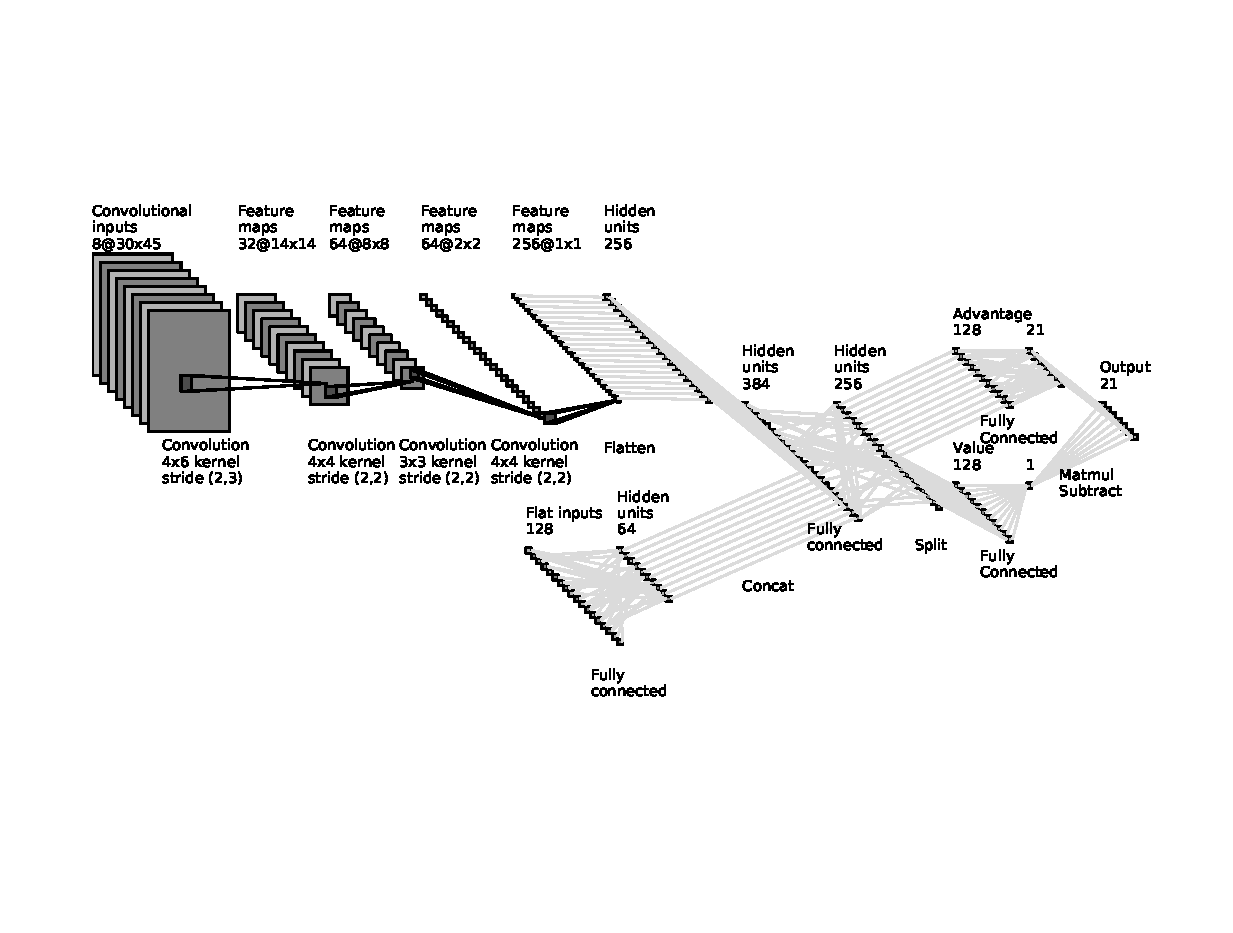
\includegraphics[trim={1.22cm 3.4cm 1.15cm 3cm},clip,width=1.02\textwidth]{draw_convnet/dqn}
	\caption{The used convolutional DQN with a dueling architecture}
	\label{fig:dqn_graph}
\end{figure}

If convolutional input is specified, four convolutional layers layers process the input to 256 feature-maps of size $1 \times 1$, which can subsequently be flattened to a one-dimensional layer. Note that there are no pooling layers in between convolutional layers. As suggested by \cite{springenberg_striving_2014}, pooling leads to a loss of localization information and can be discarded in favor of a larger \term{stride} in the convolutional layers.

\noindent While the two-dimensional \codeobj{conv\_inputs} are processed with convolutional layers, \codeobj{ff\_inputs} are fully connected to a hidden layer of variable size. This layer is concatenated to the flattened output to the convolutional layer, the result of which is densely connected to another hidden layer of 256 neurons. This layer is then, following the dueling architecture from \cite{wang_dueling_2015}, split into a separate \keyword{advantage stream} and \keyword{value stream}. While the value stream is fully connected to one hidden layer (corresponding to the state-value), the advantage ends in one output neuron for each action, which is 21 in the current implementation. The advantage stream and value stream are finally combined (as described in section~\ref{sec:dueling}) to yield 21 output neurons, corresponding to one Q-value for every action in the provided state.

Informal search led to the selection of the rectified non-linearity (\codeobj{tf.nn.relu}) as activation function as well as Adam\cite{kingma_adam:_2014} as optimizer. All weights of this network are initialized around zero (or slightly higher, to prevent \keyword{dead neurons} in combination with the relu activation-function) with only a very small standard deviation ($10^{-20}$ up to $10^{-3}$), as doing otherwise showed to impair the agent's performance after a fresh start.

In the current implementation, the DQN-model does not perform \keyword{batch normalization}\cite{ioffe_batch_2015}, as it showed to impair the agent's performance. The functions \codefunc{convolutional\_layer} and \codefunc{dense}, which are used to initialize the layers, wrap respective TensorFlow-functions and can be found in \filename{utils.py}\footnote{\url{https://github.com/cstenkamp/BA-rAIce-ANN/blob/master/utils.py}}.

The final structure of this network was subject of much experimentation. Any used hyperparameter that does not correspond to its counterpart in \cite{mnih_human-level_2015} or \cite{wang_dueling_2015} is the result of informal search, showing the best performance so far. This does by any means not mean that the parameters are optimal. Using this structure, the network performed reasonably well on given OpenAI gym-tasks, as explained earlier in this chapter.


\subsection{DDPG-model}

A DDPG-model must incorportate four ANNs to work correctly: an online- and a target version of both \codeobj{actor} and \codeobj{critic}, as found by \cite{lillicrap_continuous_2015}.  While the online networks will be used for online predictions and will be updated at every timestep, the target networks will be used for determining the directions into which the online networks should be updated. The given implementation of the \codeobj{DDPG\_model} thus \term{has} an actor and a critic, which in turn have two \codeobj{actorNet}s or \codeobj{criticNet}s, respectively. If the \codefunc{save()}-method of \codeobj{DDPG\_model} is called, it calls the respective functions of actor and critic, which save their individual variables individually. Because of that, the same critic could be used for different actors or vice versa. The information about the numbers of current inferences and others is saved in and loaded from the actor.

As the \codeobj{DDPG\_model} \term{has} \codeobj{actor} and \codeobj{critic}, it can access all their values and methods. If it accesses any of these, it specifies as argument if it wants them to internally use their online- or target network. Both actor and critic provide respective methods to update their target network.

It is not possible to use the same network structure as used in the \codeobj{DQN\_model} in any network of the \codeobj{DDPG\_model}. The actor returns continuous values which correspond directly to the action instead of a \term{softmax}-distribution over possible discrete actions. The critic needs, in contrast to the DQN-architecture, the actions as additional input to return one single Q-value. It is obvious that the \term{dueling architecture} cannot be adopted for the DDPG-critic.

In its \codefunc{q\_train\_step}-method, the \codeobj{DDPG\_model} trains both its actor and its critic by calling their respective methods -- the theoretical basis of this learning step is explained in section~\ref{ch:ddpg}, while appendix~\ref{ap:ddpg} compares the source-code to the pseudocode given in \cite{lillicrap_continuous_2015}. While normally TensorFlow minimizes losses via an optimizer (and also does so in the critic), it also allows the possibility to \codefunc{apply\_gradients}, which optimizes all elements of its respective computation graph into the direction of the supplied values. 

As the actor only needs the critic's gradients once, these can simply be passed into its \codeobj{feed\_dict}. Besides this interaction, actor and critic can be implemented completely independent of each other. In the following section, The network structure of both of them will be described individually. It is worth noting, that this model supports the usage of \keyword{TensorBoard}, and saves a summary of all its variables in a preset interval of update-steps.

\subsubsection{Network architecture}

\paragraph{Critic}

The actual computational graph of the network the \codeobj{critic} uses is specified in an extra class. In contrast to the \codeobj{DQN\_model}, it was decided to use a different class for agents that use convolutional input than for agents which do not, as informal testing showed that the \codeobj{DDPG\_model} appears to be less forgiving to changes of its network structure. This means, that the \codeobj{critic} uses a \codeobj{conv\_criticNet} if \codeobj{agent.usesConv} and a \codeobj{lowdim\_criticNet} otherwise.

In contrast to the model of a DQN, the critic gets a state and an action as input, returning a single estimate of the respective state-action value \term{Q}. Like a DQN however, it is trained using temporal differences, requiring a better estimate of each Q-value to update its parameters. As however only the online network is updated this way (whereas the target-network receives smooth updates), the \codeobj{placeholder} to hold these is specified in the class \codeobj{Critic}, not in one of its used networks. The \codeobj{Critic}-class further specifies a function to return the \codefunc{action_gradiens(inputs, actions)} for the \codeobj{actor}.

The network-architecture of the convolutional critic is specified in figure~\ref{fig:2dcrit}. 

\begin{figure}[h]
	\centering 
	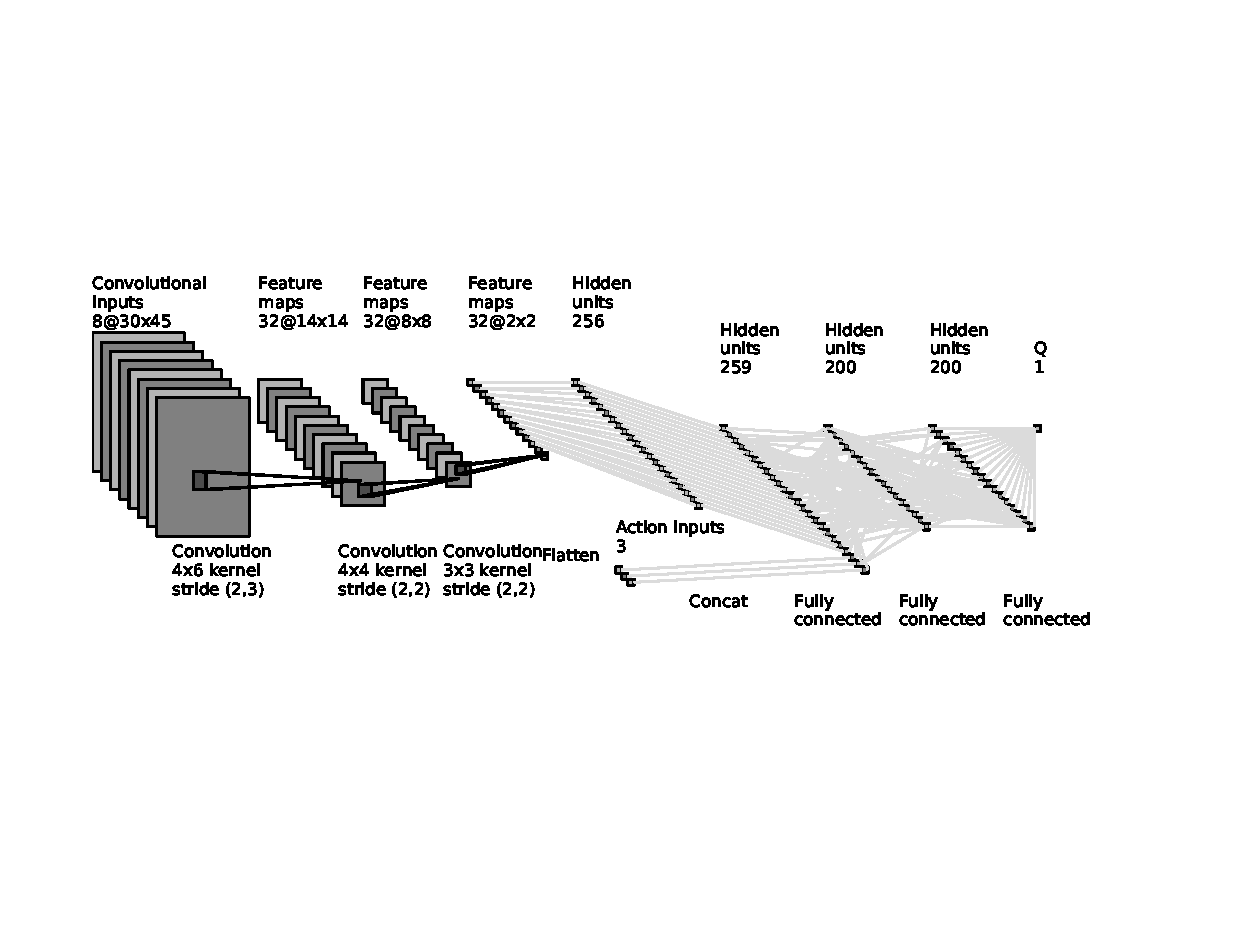
\includegraphics[trim={1.22cm 4.6cm 2cm 3cm},clip,width=1.05\textwidth]{draw_convnet/critic-2d}
	\caption{Convolutional critic}
	\label{fig:2dcrit}
\end{figure}

The number of input-maps is variable, however the kernel size and stride of the convolutional layers are adjusted for an input-size of $30\times45$ pixels to create 32 $2\times2$ feature maps in three convolutional layers (again, pooling layers were dropped in favor of higher stride).  Afterwards, the feature maps are flattened into a layer of 256 hidden units, to which the 3 action-inputs are concatenated. This layer is densely connected to two other hidden layers of 200 units, which ultimately leads to one output-neuron: the Q-value.\\

\noindent The network-architecture of the low-dimensional critic (\codeobj{lowdim\_criticNet}) is depicted in figure~\ref{fig:lowdcrit}.

\begin{figure}[h]
	\centering 
	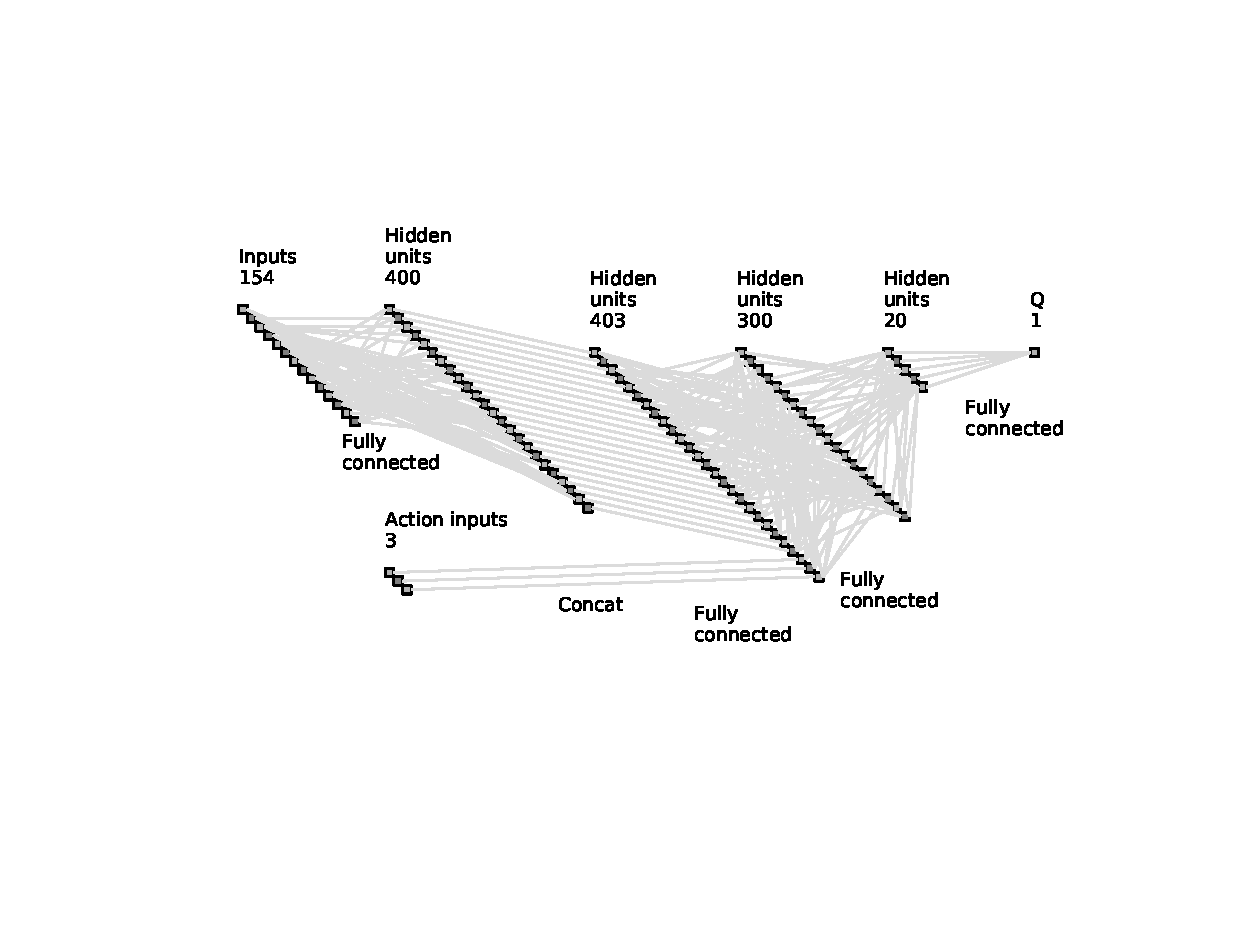
\includegraphics[trim={3.7cm 4.4cm 2cm 3cm},clip,width=.98\textwidth]{draw_convnet/critic-lowd}
	\caption{Low-dimensional critic}
	\label{fig:lowdcrit}
\end{figure}

The number of input-neurons the low-dimensional critic uses is variable depending on the agent -- for the \filename{ddpg\_novison\_rl\_agent} it consisted of 154 inputs. These are densely connected to a layer of 400 hidden units, to which the 3 action-inputs are concatenated. This layer of 403 units is fully connected to another hidden layer of 300 units, which is connected to a layer of 20 hidden units. This final hidden layer is connected to the output-layer specifiying the Q-value.

As suggested by \cite{lillicrap_continuous_2015}, both variants of the critic use $L2$ weight decay for all their layers. Furthermore, the implementation allows to use \keyword{batch normalization}\cite{ioffe_batch_2015}, which can be toggled for each layer individually with a respective argument. In the original DDPG-algorithm, the authors used this technique in order to use the same network hyperparameters for differently scaled input-values. In the learning step when using minibatches, \batchnorm normalizes each dimension across the samples in a batch to have unit mean and variance, whilst keeping a running mean and variance to normalize in non-learning steps. In Tensorflow, batchnorm can be added with respective additional layers and one additional input that specifies the phase (learning step/non-learning step)\footnote{for further information, see \url{https://www.tensorflow.org/api\_docs/python/tf/contrib/layers/batch_norm} [accessed on 5th September, 2017]}. Though \cite{lillicrap_continuous_2015} report success on using batch normalization, in practice it often leads to instability. After much informal it turned out that using \batchnorm in the critic only harms the performance by giving a very small and similar Q-value for all states, which is why it is deactivated in the final implementation.

\noindent All layers are summarized with the function \codefunc{variable\_summary} from \filename{utils.py}, writing their summary to a file that can be inspected by \term{TensorBoard} every \codeobj{conf.summarize\_tensorboard\_allstep} steps. 


\paragraph{Actor}

Just like the \codeobj{critic}, the \codeobj{actor} uses a \codeobj{conv\_actorNet} if \codeobj{agent.usesConv} and a\\ \codeobj{lowdim\_actorNet} otherwise.

The network architecture of the high-dimensional critic can be inspected in figure~\ref{fig:2dact}. Its structure is similar to that of the high-dimensional critic, with the difference that the actor does not take the actions as input, but connects the last hidden layer to three output neurons, corresponding to the values for the three actions. This \keyword{Outs}-layer is scaled afterwards to yield the \keyword{ScaledOuts}-layer. All hidden units but the last use a \codeobj{tf.nn.relu} activation function, whereas the last uses a \codeobj{tanh}-activation-function. While $tanh$ has a range of $[-1,1]$, the actions may have a different range (e.g. $acceleration \in [0,1]$). The final scaling layer adjusts the range correspondingly.

\begin{figure}[h]
	\centering 
	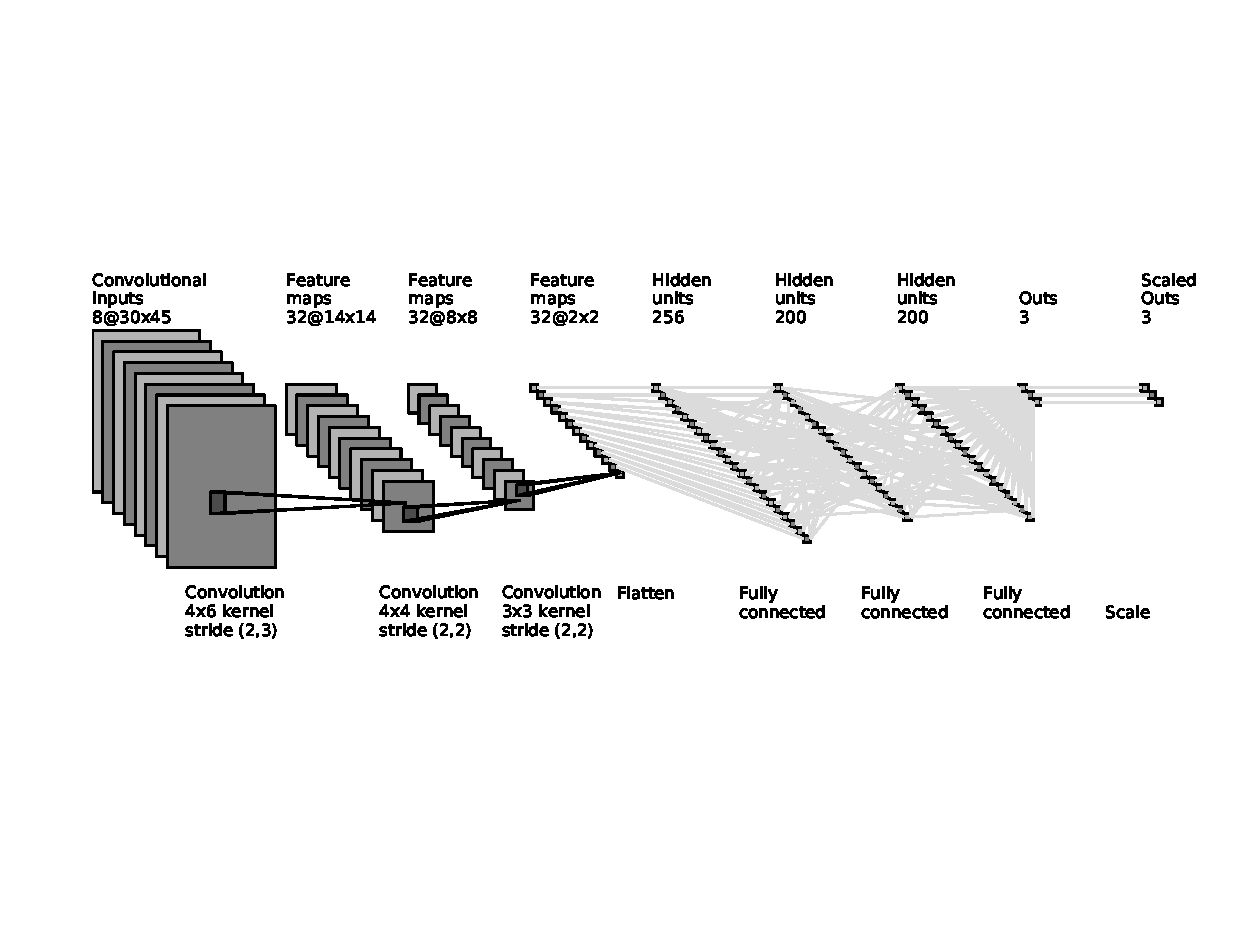
\includegraphics[trim={1.22cm 5.03cm 0.4cm 3cm},clip,width=1.01\textwidth]{draw_convnet/actor-2d}
	\caption{Convolutional actor}
	\label{fig:2dact}
\end{figure}

The structure of the low-dimensional actor (figure~\ref{fig:lowdact}) is fairly simple. The inputs are fully connected to 300 hidden units, which are fully connected to another 200 hidden units, which is in turn connected to the output-units, which are scaled again as in the convolutional case. 

\begin{figure}[h]
	\centering 
	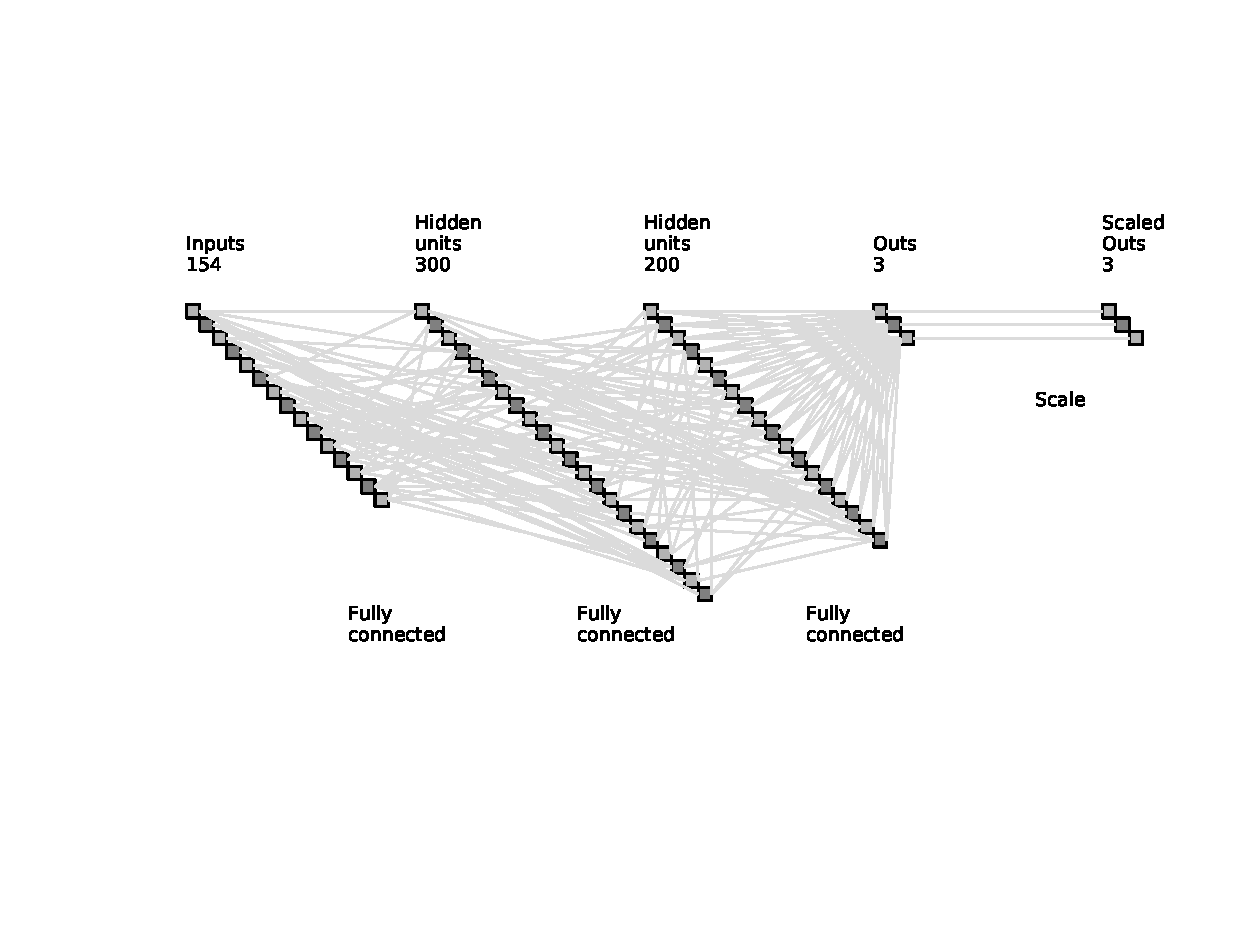
\includegraphics[trim={2.7cm 4.2cm 0.8cm 3cm},clip,width=1.01\textwidth]{draw_convnet/actor-lowd}
	\caption{Low-dimensional actor}
	\label{fig:lowdact}
\end{figure}

In contrast to the critic, the actor does not use $L2$ normalization, as suggested by \cite{lillicrap_continuous_2015}. Informal testing showed, that \batchnorm indeed helps convergence in the actor, which is why it is enabled for all fully-connected layers. Besides the critic's preterminal layer, all hyperparameters correspond roughly to \cite{lillicrap_continuous_2015}, with all differences being the result of informal testing. As in the DQN-model, the rectified non-linearity (\codeobj{tf.nn.relu}) serves as activation function and Adam\cite{kingma_adam:_2014} as optimizer. The convolutional layers are implemented using \codeobj{conv2d} from TensorFlow's \codeobj{slim} package. All layers that are recorded for TensorBoard are added to the collection \codeobj{summaryOps}.

Like the DQN-model, this model also incorporates a function that forces the model to accelerate if the \codeobj{stands\_input} is set to \codeobj{true}. This is however implemented differently, as it is not necessary to change the Q-value of actions because the output of the actor can be changed instead. If the corresponding variables \codeobj{conf.use\_settozero} and \codeobj{stands\_input} are \codeobj{true}, the value for the $brake$ is simply set to zero, whereas the value for $throttle$ is set to a random value of at least $0.5$. 

Further, the DDPG-model also manually forbids simultaneous braking and accelerating. In contrast to the DQN-model however, no combined action is returned, but an individual value for $throttle$ and $break$. In the method \codefunc{apply\_constraints}, the actor checks if both values are simultaneously above $0.5$, and randomly sets one of those to a random value below $0.5$ if so.

Agents that use the DDPG-model must overwrite the functions \codefunc{makeNetUsableAction} to account for the fact the DDPG-model works with un-discretized action and needs these as input to perform its learning step. 
It was further mentioned in section~\ref{sec:contexptheory} that an agent using a continuous model works better with noisy actions instead of completely random actions as exploration function. To do so, a method like \codefunc{make\_noisy}, and the change the implemented \codefunc{randomAction(gameState)} are required.

%############################################################################################
\section{Implemented agents}
%############################################################################################

In the course of this thesis, five different agents were implemented to both demonstrate how to use the given framework and answer the research questions stated in section~\ref{sec:researchquestions}.  The following table shows their names and distinctive properties: 

\begin{flushleft}
\begin{tabular}{l l l l}
	filename & uses model & uses visionvector & performs RL\\
	\hline
	\textbf{ddpg\_novision\_rl\_agent}.py\footnote{\url{https://github.com/cstenkamp/BA-rAIce-ANN/blob/master/agents/ddpg_novision_rl_agent.py}} & DDPG & no & yes\\	
	\textbf{ddpg\_rl\_agent}.py\footnote{\url{https://github.com/cstenkamp/BA-rAIce-ANN/blob/master/agents/ddpg_rl_agent.py}} & DDPG & yes & yes\\
	\textbf{dqn\_novision\_rl\_agent}.py\footnote{\url{https://github.com/cstenkamp/BA-rAIce-ANN/blob/master/agents/dqn_novision_rl_agent.py}} & DQN & no & yes\\
	\textbf{dqn\_rl\_agent}.py\footnote{\url{https://github.com/cstenkamp/BA-rAIce-ANN/blob/master/agents/dqn_rl_agent.py}} & DQN & yes & yes\\
	\textbf{dqn\_sv\_agent}.py\footnote{\url{https://github.com/cstenkamp/BA-rAIce-ANN/blob/master/agents/dqn_sv_agent.py}} & \blap{supervised network\\ with DQN-structure} & yes & no\\[2em]
\end{tabular}
\end{flushleft}

The agents differ in the used \keyword{model} (and through that their \keyword{exploration-function}), their \keyword{observation function}, and if and how they incorporate \keyword{pretraining}. The UML-diagram in figure~\ref{fig:umlAgents} shows the attributes and methods that the respective actions overwrite (note however that it is incomplete and for example does not show the functions that are overwritten to incorporate a GUI). All agents end a training episode after crashing into a wall, completing a lap, turning around or after $60$ seconds driving-time without either of those.

\begin{figure}[h]
	\centering 
	\includegraphics[width=\textwidth]{uml_diagrams/agent_inText.2}  
	\caption[UML-Diagram of the implemented agents and their superclasses]{(incomplete) UML-Diagram of the five implemented agents and their abstract superclasses}
	\label{fig:umlAgents}
\end{figure}

In the following sections, these functions will be described. Further, the used reward function will be elucidated, even though it is the same for all agents. To specify which agent a \term{feature} belongs to, captions will indicated the respective agents. If no such caption is given, it is assumed that all agents use the same feature.

\subsection{Pretraining}

\label{sec:pretrainingcode}

The exported \codeobj{.svlap}s from Unity are used to train an agent. Note however, that only complete, \codeobj{valid} laps are exported. This guarantees that no laps where the car steeres into the wall or drives too slow will be in the sample. It can thus also be safely assumed that all datapoints in the set are \textit{good}, in the sense of contributing to relatively fast lap. 

To assess the quality of a pre-training, the model's method \codefunc{getAccuracy} is used. The \keyword{accuracy} as defined by this method is the percentage of all calculated actions that result in the same discretization than their counterpart from the dataset. While for the DDPG-model, another way of assessing the accuracy using gaussian distances could be used, it will not be considered in the remainder of this thesis when talking about \textit{accuracy}.

\subsubsection{\term{dqn\_sv\_agent}}

Using only good datapoints is perfectly suited for supervised training, where the agent learns to do the same actions as provided in the dataset. The \filename{dqn\_sv\_agent} simply iterates over the dataset for a specified number of iterations, splitting the dataset into minibatches according to its settings. To do so, this agent specifies the \codefunc{preTrain}-function itself, as it is not specified in its only superclass, \codeobj{AbstractAgent}.

The original definition of an agent's observation-function included, following \cite{mnih_human-level_2015}, the last actions an agent performed. Interestingly however, agents that included the action learned an action solely in dependance of this input. This can be explained due to a huge portion of consecutive actions being equal (for example when driving a straight track). Because of this, the previous actions were removed as part of the observation for all agents.

The implementation forbids to use an agent that performed supervised pre-training to subsequently perform reinforcement learning, as it does not make sense to re-use an agent that trained supervisedly for q-learning. While a supervisedly trained agent may select the same actions than a q-learning correspondance, it does not ascribe any Q-values to these actions. As long as the $argmax$ is the same, it does not matter for a supervisedly trained agent what the respective value of all actions are. As the $argmax$-operation is for example invariant to equal scaling of all actions, it is obvious that the chance that the respective activations correspond to actual q-values is extremely slight.

\subsubsection{Other agents}

While it is good for a supervisedly trained agent to learn only from good actions, the same cannot be said for q-learning agents. As mentioned before, q-training is normally used when the state dynamics of the underlying environment is unknown. To learn accurately, a q-learning agent must thus get \textit{representative} samples of the environment. The actions in the dataset used for pretraining are all parts of \textit{good} rounds, where the car mostly drives at high speeds and does not crash into a wall. It is easy to see, that using only those samples is not representative about the environment. Almost all values in the dataset are likely to have high rewards. If a q-learning agent is trained purely on samples with a high reward, it will assume that high rewards are representative for the entire environment and assign a high reward to all those state-action pairs. Testing showed that this was actually the case, and that an agent trained this way did not learn at all. Because of this, in the \codefunc{preTrain}-function of \codeobj{AbstractRLAgent}, the method \codefunc{make\_trainbatch} (printed in algorithm~\ref{alg:maketrainbatch}) is used.

\begin{algorithm}[h]
\begin{lstlisting}[language=Python, style=Python, frame=none]
def make_trainbatch(self,dataset,batchsize,epsilon):
	trainBatch = dataset.create_QLearnInputs_fromBatch(*dataset.next_batch(self.conf, self, batchsize), self)
	s,a,r,s2,t = trainBatch
	if np.random.random() < epsilon:
		r = np.zeros_like(r)
		a = np.array([random_unlike(i,self) for i in a])
		t = np.array([True]*len(t))
		trainBatch = s,a,r,s2,t
	return trainBatch
\end{lstlisting}%
\caption{The \codefunc{make\_trainbatch} - function}
\label{alg:maketrainbatch}
\end{algorithm}

This function inflates the dataset, by adding state-action combinations that were not originally in the dataset with a respective reward of zero. Testing showed that training worked best if 80\% percent of those fake-actions were included.

In the case of discrete actions, $a$ is saved as the $argmax$ of the one-hot vector. In this case, the method \codefunc{random\_unlike} returns an index dissimilar from that argmax. In the case of continuouous actions, the action is discretized first, and the result afterwards dediscretized. While it was tried to instead add gaussian noise to the action while diminishing the reward only according to the gaussian distance of these two actions, testing showed no success for this approach.

This method simulates an environment that rewards the actions from the pretraining as demanded and provides a reward of zero for any other action. Using this method makes it possible to archieve reasonable accuracies with q-pretraining, where at least the performed action gets ascribed a correct Q-value. 

Unfortunately, reinforcement learning agents that used pre-training in this fashion were still not able to correctly make use of it, as figure~\ref{sec:incorporatePre} will show.

\subsection{Exploration}

An agent uses an exploration function to learn about different states. As a supervised agent does not learn about the environment at all, it does not incorporate an exploration function.

\subsubsection{\term{dqn\_rl\_agent} and \term{dqn\_novision\_rl\_agent}}

As the model of DQN-based agent discretizes the action into one unique value, so does its exploration function. Both agents use the \codefunc{randomAction}-method as provided in \codeobj{AbstractRLAgent}. As the \codeobj{randomAction}-method is called with a probability of $\epsilon$ and otherwise the greedy result of \codeobj{policyAction}, their exploration algorithm corresponds to the standard $\epsilon$-greedy approach.

The \codefunc{randomAction} itself selects an action purely by chance, while forbidding simultaneous activation of throttle and brake and forcing a throttle if the car stands.

Even though it was not done for these agents, it would also be possible to incorporate higher-level information into the \codefunc{randomAction}-function. As the values required by the environment are continuouos, the method could for example use the result of \codefunc{policyAction} and apply noise to it or select actions basing on the Boltzmann-exploration function. It is an open question how this would manifest in the performance of these agents.

\subsubsection{\term{ddpg\_rl\_agent} and \term{ddpg\_novision\_rl\_agent}}

As for DDPG-based actions it holds that $action \subset \mathds{R}^{n \in \mathds{N}}$, which makes it natural that their \codefunc{randomAction} also returns continuous values. For exploration the straightforward approach is to add some noise to their \codefunc{policyAction}. As explained in section~\ref{sec:contexptheory} and \cite{wawrzynski_control_2015}, pure random noise leads to very jerky behaviour, which is unrealistic for the given simulation. Because of that, temporal correlation is incorporated with an  Ornstein-Uhlenbeck process.

Modelling noise with an Ornstein-Uhlenbeck process changes the standard framework for $\epsilon$-greedy, as no completely random actions are taken anymore. Because noise is added to the result of a networks inference in all inferences, the method \codefunc{randomAction} is overwritten to return the value of \codefunc{policyAction}.  The parameter \codeobj{epsilon} is incorporated nevertheless, to control how much noise influences the action of \codefunc{policyAction}. This method calculates every action according to its model, and then uses a \codefunc{make\_noisy}-function to add the temporally correlated noise to its result, as defined in section~\ref{sec:contexptheory}. The method \codefunc{make\_noisy} is further specified in algorithm~\ref{alg:ornstein}, inclusive the values for the Ornstein-Uhlenbeck as they resulted from testing.

In this method, the values for $\mu$, $\Theta$ and $\sigma$ are different for all three actions. A relatively high mean value $\mu$ for the throttle together with a low $\mu$ for the brake ensures that the car will have a high prior probability to accelerate the car, instead of standing a lot which would cripple exploration. A lower $\Theta$ for the steering ensures that the temporal correlation is more relevant than reverting to the mean.

Note that an agent that uses an Ornstein-Uhlenbeck exploration function must specify a \codeobj{\_noiseState} variable, which is reset as soon as an episode ends.

\begin{algorithm}[h]
	\begin{lstlisting}[language=Python, style=Python, frame=none]
self.OU_mu = [0.5, 0.05, 0.0]
self.OU_theta = [0.85, 0.85, 0.6]
self.OU_sigma = [0.1, 0.05, 0.3]

def make_noisy(self, action):
	def Ornstein(x,mu,theta,sigma):
		return theta * (mu - x) + sigma * np.random.randn(1)
	self._noiseState[0] = Ornstein(self._noiseState[0],  self.OU_mu[0] , self.OU_theta[0], self.OU_sigma[0])
	self._noiseState[1] = Ornstein(self._noiseState[1],  brakemu,        self.OU_theta[1], self.OU_sigma[1])  
	self._noiseState[2] = Ornstein(self._noiseState[2],  self.OU_mu[2] , self.OU_theta[2], self.OU_sigma[2])
	action[0] += self.epsilon * self._noiseState[0]
	action[1] += self.epsilon * self._noiseState[1]
	action[2] += self.epsilon * self._noiseState[2]
	action = np.array([clip(action[i],self.conf.action_bounds[i]) for i in range(len(action))])
	return action
	\end{lstlisting}%
	\caption{Ornstein-Uhlenbeck process to generate noisy actions}
	\label{alg:ornstein}
\end{algorithm}


\subsection{Reward}
		
\label{sec:reward}		
		
The success of a reinforcement learning agent hinges critically on its reward function. Especially in the domain of virtual racing simulations, there is much debate about what serves as a good reward. As listed in section~\ref{sec:relatedimplements}, the original DDPG-paper \cite{lillicrap_continuous_2015} used the car's velocity in direction of the street as reward. Applying this reward-function to the given progress did not lead to success (as figure~\ref{fig:dqnrewardspeedstuff} shows). If only speed is rewarded, the car accelerates as much as possible and simply crashes into the wall at the first turn. In this implementation -- as well as in many others -- accelerating as much as possible is not the correct behaviour. In theory, a reinforcement learning agent should learn to accept a smaller reward in the current state in favor of a more desirable follow-up state, however no agent seemed to have explored enough to learn that other possibilities besides the unevitable crash into the wall are possible by braking for a consecutive number of frames. 

To create an agent that learns successfully, a reward-function must thus be implemented that rewards the \textit{correct} behaviour at any time, including braking. Consequently, it was decided to implement a reward function that rewards high speeds only if no sharp turn is ahead, and punishes them otherwise. The resulting definition uses \codeobj{OtherInputs.WallDistVec[6]} (corresponding to the grey line in figure~\ref{fig:walldistvec}) to measure the distance to the closest wall ahead of the car. The employed function to calculate the reward is specified in algorithm~\ref{alg:speedinrelationto}. A visualization of its value in dependence of speed and wall-distance can further be found in plot \textbf{D} of figure~\ref{fig:reward}.


\begin{algorithm}[h]
	\begin{lstlisting}[language=Python, style=Python, frame=none]
vvec1_hist, vvec2_hist, otherinput_hist, action_hist = gameState
reward = otherinput_hist[0].WallDistVec[6]-otherinput_hist[0].SpeedSteer.speedInStreetDir+(80/250)
reward = 1-(abs(reward)*3) if reward < 0 else (1-reward)+0.33
reward = min(1,reward)
reward += 0.3*otherinput_hist[0].SpeedSteer.speedInStreetDir
	\end{lstlisting}%
	\caption{Rewarding speed in relation to the wall-distance}
	\label{alg:speedinrelationto}
\end{algorithm}

While an agent using purely this reward definition performed much better than one using only the speed, it turned out that adding other components to the reward optimized the performance and tempo of learning even more. Figure~\ref{fig:reward} visualizes some other components that were additionally used, with the source code to caluclate those in appendix~\ref{AppendixD}

\begin{figure}[h]
	\centering 
	\begin{annotatedFigure}
		{\includegraphics[trim={5.5cm 1cm 4.5cm 2cm},clip,width=1\textwidth]{reward_components}}
		\annotatedFigureBox{0.052,0.93}{0.052,0.93}{A}{0.052,0.93}%bl
		\annotatedFigureBox{0.395,0.93}{0.395,0.93}{B}{0.395,0.93}%bl
		\annotatedFigureBox{0.74,0.93}{0.74,0.93}{C}{0.74,0.93}%bl
		\annotatedFigureBox{0.052,0.45}{0.052,0.45}{D}{0.052,0.45}%bl
		\annotatedFigureBox{0.4,0.45}{0.4,0.45}{E}{0.4,0.45}%bl
		\annotatedFigureBox{0.74,0.45}{0.74,0.45}{F}{0.74,0.45}%bl
	\end{annotatedFigure}
	\caption{Reward-components}
	\label{fig:reward}
\end{figure}

Plot \textbf{A} shows the sub-component of rewarding the car's \textit{traverse position}. As it is reasonable for the car to stay on the street (less slip and better control), doing so is rewarded. As long as the car stays on the street, it receives the full reward, whereas this reward decreases steeply from the \textit{curb} on.

Another component is the \textit{Minimum-Speed-Reward} (plot \textbf{C}): It is easily possible to keep a constant speed at all times. To ensure that driving to slow is punished, this function subtracts a value for speeds lower than $20\%$ of the maximally possible speed. As the function from algorithm~\ref{alg:speedinrelationto} sometimes rewards very low speed, it is useful to combine it with this component to discourage too slow speeds.

If the \keyword{carAngle} is too big, it is also rewarded to steer back into the direction that decreases this angle. As the purpose of this component is to make the car steer back to the street if it is too close to a wall, this reward is only relevant if the traverse position of the car indicates that it is close to a wall. Plot \textbf{E} shows the preliminary steering-reward in dependence of car-angle and steering-command, and plot \textbf{F} shows the actually resulting reward, depending on the result from \textbf{E} and the car's traverse position. This steer-bonus is stated in lines 19-26 of the source code in appendix~\ref{AppendixD}. 

Note that a reward function must not provide more reward to get out of an undesired situation as it gives for not getting into such a situation in the first place, as that would lead to an agent intentionally generating the undesired situation.

These components are not all that are used in the final agent, but listing all of them would be beyond the scope of this thesis. The interested reader is therefore referred to appendix~\ref{AppendixD}, where the source-code of this function is given.

The actual reward is a weighted sum of all these components, with the respective weights being a result of informal testing. Note that the final result is clipped as \codeother{reward = max(0, reward)}. It is a well-known fact that negative rewards impair the behaviour of an agent more than they help. If for example the reward for being too far off-center is all negative, then the car would get a higher cumulative when it ends the episode by driving into a wall. Testing confirmed this scenario. To prevent such scenarios, all rewards but the one that ends the episode must be positive.


\subsection{Observation}

\label{sec:observation}

An agent's observation-function is specified in its method \codefunc{getAgentState(gameState)}, which creates the \codeobj{agentState} used for its model and its memory from the \codeobj{gameState}. \codeobj{AbstractAgent} specifies an observation-function that can be used by sub-classes. This function is only overwritten by the agents termed $novision$-agents, specifically the \term{ddpg\_novison\_rl\_agent} and the \term{dqn\_novision\_rl\_agent}.

\subsubsection{\term{ddpg\_rl\_agent}, \term{dqn\_rl\_agent} and \term{dqn\_sv\_agent}}

These agents use the result of both minimaps (see section~\ref{ch:thevectors}) in their definition of agent-state. As suggested by \citet{mnih_human-level_2015}, an agent uses the \term{M} most recent states as its observation, with \term{M} (\codeobj{config.history\_frame\_nr}) set to four. This ensures that the agent has a way of inferring trajectories from the static images. While this should in theory be enough to calculate the current velocity, testing showed that additionally passing the current velocity improved the accuracy on a supervised test set. Note that this velocity is passed to the network in the form of a vector instead of a single number.

The actual two-dimensional input to a network of this form does not consist of four feature maps, but of eight, as both mini-maps are stacked before handing it in as input. Both maps are provided in the hope that one of them provides a coarse overview, whereas the other helps precise navigation. Note that the mini-maps record mostly the track in front of the car, not the surroundings of it.

While in the original DQN as put forward by \citet{mnih_human-level_2015} its last actions are also input to the agent, this is removed in the current version of the implementation. Supervised testing showed, that an agent only learns to repeat its last action -- which is the correct behaviour in a high percentage of cases, but does not generalize at all when applied to new scenarios. As further testing showed that there seemed to be no benefit of providing the action altogether, it was decided to remove this input from the agent's observation in all scenarios. It is however possible to change that back by uncommenting the respective line in \codefunc{AbstractRLAgent.getAgentState}.

Note that as mentioned before, an agent's state treates the convolutional input (the minimaps) separately from the other inputs, which in this case consists only of the speed. The third information of an agent's state is the information whether a car stands to forbid braking -- according to this observation-function, this input is \codeobj{true} if the car drives slower than $4\%$ of its maximum-speed, corresponding to roughly $6km/h$.

\subsubsection{\term{ddpg\_novison\_rl\_agent} and \term{dqn\_novision\_rl\_agent}}

The observation of the $novision$-agents does not use the minimaps, to save on memory required for the replay buffer. Because of that, the respective convolutional input of the \codeobj{agentState} is \codeobj{None}. To make up for that loss, the agent instead uses a low-level information. As the provided information is already explained in section~\ref{ch:thevectors}, a numeration of the used vectors must suffice here:
\begin{itemize}[noitemsep]
	\item CenterDistVec
	\item values $5-11$ from SpeedSteer 
	\item StatusVector
	\item WallDistVec
	\item LookAheadVec
\end{itemize}

All of these input-values are scaled to a range of $[0,1]$, such that values on a naturally high scale do not influence the agent's policy out of proportion.

Note, that these agents also do not provide the past action, with similar reasoning than above. Testing even showed that providing the motor torque and steer information (values 1-4 from \textit{SpeedSteer}) is just as destructive: If this vector was provided, an agent learned to hit the throttle if the motor torque was already high, and to simply steer into the same direction as the frame before, which lead to the car driving right into the wall as fast as possible. Removing these elements from an agent's observation was a necessary condition for a capable policy.

While \textit{WallDistVec} and \textit{LookAheadVec} provide information of the course of the track in front of the car, it does (just like the mini-maps) not provide information about the course of the track to the side of the car. Incorporating fixed range-finder sensors, as suggested by \cite{loiacono_simulated_2013}, may be a worthy addition in future implementations.